
\begin{titlepage}
\begin{center}

\begin{minipage}{0.2\linewidth}
    \begin{flushleft}
        \begin{figure}[H]
    		
\includegraphics[scale=0.21]{Imagens/LOGO-UNICAMP.png}
    	\end{figure}
    \end{flushleft}
\end{minipage}
\begin{minipage}{0.5\linewidth}
	\begin{center}
		
		Universidade Estadual de Campinas
		
		Instituto de Computação
		
		MO601 – Arquitetura de Computadores II

		Prof. Rodolfo Jardim de Azevedo
		
	\end{center}
\end{minipage}
\begin{minipage}{0.25\linewidth}
    \begin{flushleft}
        \begin{figure}[H]
    		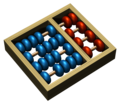
\includegraphics[scale=0.6]{Imagens/logo-ic-unicamp-slant-tint-beg-sky-ora-0120.png}
    	\end{figure}
    \end{flushleft}
\end{minipage}

\vfill


{\fontsize{28}{\baselineskip}\selectfont
Projeto 1
}

\vfill




{\fontsize{36}{\baselineskip}\selectfont
Um simulador super básico de circuitos lógicos
}

\vfill



{\fontsize{20}{\baselineskip}\selectfont
Rubens de Castro Pereira

RA: 217146
}


% \begin{minipage}{0.7\linewidth}
% 	{\onehalfspacing\fontsize{20}{\baselineskip}\selectfont
	
%     Rubens de Castro Pereira
    
    
    
%     }
% \end{minipage}
% \begin{minipage}{0.25\linewidth}
% 	{\onehalfspacing\fontsize{20}{\baselineskip}\selectfont
% 	RA: 217146
	
	
	
% 	}
% \end{minipage}

\vfill





{\fontsize{14}{\baselineskip}\selectfont
	Campinas - SP

	\today
}

\end{center}
\end{titlepage}